\باب{بنیادی حساب}
	ثنائی نظام میں حساب بالکل اسی طرح کیا جاتا ہے جس طرح عشری  نظام میں۔چند مثالوں کے مطالعہ سے وضاحت ہو گی۔
	
	ثنائی نظام میں اعداد کا مجموعہ اعشاری نظام میں دو اعداد کے مجموعہ سے سمجھا جا سکتا ہے۔اعشاری نظام کی مندرجہ ذیل مثال پر غور کریں جس میں \عددی{37.5} اور \عددی{29.6} جمع کیے گئے ہیں۔
\begin{center}
\begin{otherlanguage}{english}
\begin{tabular}{R}
11\phantom{.5}\\
37.5\\
+29.6\\
\midrule
67.1
\end{tabular}
\end{otherlanguage}
\end{center}
آپ نے دیکھا کہ حاصل\عددی{(1)} کو (بائیں) زیادہ وزنی مقام پر منتقل کیا گیا۔یہی ثنائی جمع میں کیا جائے گا۔ ثنائی نظام میں صرف دو ہندسے، \عددی{0} اور \عددی{1}، پائے جاتے ہیں جن کی چار ممکنہ مجموعے درج ذیل ہیں۔
\begin{center}
\begin{otherlanguage}{english}
\begin{tabular}{L}
\phantom{1}1\\
\phantom{+}1\\
+1\\
\midrule
\phantom{1}10
\end{tabular}\quad\quad
\begin{tabular}{L}
\phantom{11}\\
\phantom{+}1\\
+0\\
\midrule
\phantom{1}01
\end{tabular}\quad\quad
\begin{tabular}{L}
\phantom{11}\\
\phantom{+}0\\
+1\\
\midrule
\phantom{1}01
\end{tabular}\quad\quad
\begin{tabular}{L}
\phantom{11}\\
\phantom{+}0\\
+0\\
\midrule
\phantom{1}00
\end{tabular}
\end{otherlanguage}
\end{center}

پہلی تین جمع میں حاصل \عددی{0} جبکہ آخری میں حاصل \عددی{1} ہے۔

آئیں، زیادہ ثنائی ہندسوں کے اعداد کی جمع کی مثالیں دیکھیں؛ ان کی اعشاری نظام میں جمع بھی دی گئی ہیں۔
\begin{center}
\begin{otherlanguage}{english}
\begin{tabular}{L}
\phantom{+}1\phantom{5}\\
\phantom{+}13\\
+09\\
\midrule
\phantom{+}22_{10}
\end{tabular}\quad\quad
\begin{tabular}{L}
\phantom{1}1\phantom{11}1\\
\phantom{+}1101\\
+1001\\
\midrule
\phantom{1}10110_2
\end{tabular}\quad\quad
\begin{tabular}{L}
\phantom{11}\\
\phantom{+}3\\
+2\\
\midrule
\phantom{+}5_{10}
\end{tabular}\quad\quad
\begin{tabular}{L}
\phantom{1}1\\
\phantom{+}11\\
+10\\
\midrule
\phantom{1}101_2
\end{tabular}
\end{otherlanguage}
\end{center}

دائیں ہاتھ ثنائی \عددی{11} اور \عددی{10} جمع کر کے \عددی{101_2} حاصل کیا گیا جو اعشاری نظام میں \عددی{3+2=5}ہو گا، جبکہ بائیں ہاتھ ثنائی \عددی{1101} اور \عددی{1001} جمع کر کے \عددی{10110_2} حاصل کیا گیا جو اعشاری نظام میں \عددی{13+9=22} کے مترادف ہے۔

آخر میں، کسری اعداد کی جمع کی ایک مثال دیکھتے ہیں۔
\begin{center}
\begin{otherlanguage}{english}
\begin{tabular}{L}
\phantom{+}1\phantom{.75}\\
\phantom{+}5.75\\
+3.50\\
\midrule
\phantom{+}9.25_{10}
\end{tabular}\quad\quad
\begin{tabular}{L}
\phantom{+}111\phantom{.11}\\
\phantom{+}101.11\\
+\phantom{1}11.10\\
\midrule
\phantom{1}1001.01_2
\end{tabular}
\end{otherlanguage}
\end{center}

\حصہ{ثنائی نظام میں اعداد منفی کرنا}
دو بِٹ (ثنائی عدد) منفی کرنے کے درج ذیل چار ممکنات پائے جاتے ہیں۔
\begin{align*}
0-0&=0\\
1-0&=1\\
1-1&=0\\
0-1&=1 \quad \text{\RL{\small{(ادھار ایک)}}}
\end{align*}
ی آخری مساوات میں صفر سے ایک اس صورت منفی کیا دکھایا گیا ہے جب ادھار \عددی{1} لینا ممکن ہو۔ایک اور مثال دیکھتے ہیں۔
\begin{center}
\begin{otherlanguage}{english}
\begin{tabular}{L}
\phantom{-}6.25\\
-5.50\\
\midrule
\phantom{-}0.75_{10}
\end{tabular}\quad\quad
\begin{tabular}{L}
\phantom{-}110.01\\
-101.1\\
\midrule
\phantom{-11}0.11_2
\end{tabular}
\end{otherlanguage}
\end{center}

ثنائی منفی کی چند مثالیں حل کر کے اعشاری منفی سے ان کی تصدیق کریں۔ ایسا کرنے سے زیادہ وضاحت ہو گی۔



\حصہ{اساسی تکملہ یا \عددی{r} کا تکملہ}
کسی بھی اساسی نظام میں، ہندسہ کو اساس ، \عددی{(r)}، سے منفی کرنے سے ہندسے کا  \اصطلاح{اساسی تکملہ }\فرہنگ{اساسی تکملہ} (یا \عددی{r} کا تکملہ) حاصل ہو گا۔یوں، ہندسہ اور ہندسے کے اساسی تکملہ کا مجموعہ اساس کے برابر ہو گا۔مثلاً، اعشاری نظام میں \عددی{3} کا اساسی تکملہ \عددی{10-3=7} (یا \عددی{7} کا اساسی تکملہ \عددی{3} )   ہے اور ان دونوں کا مجموعہ \عددی{3+7=10} اعشاری نظام کے اساس کے برابر ہے۔اسی طرح \عددی{5} کا اساسی تکملہ \عددی{5}، اور \عددی{9} کا اساسی تکملہ \عددی{1} ہو گا۔

درج بالا مثالوں سے واضح ہے کہ کسی بھی ہندسہ (مثلاً \عددی{3}) کے اساسی تکملہ (یعنی \عددی{7}) کا اساسی تکملہ وہی ہندسہ (یعنی \عددی{3}) ہو گا۔ 

اساسی تکملہ کے تصور کو ایک سے زائد ہندسوں پر مبنی عدد تک وسعت دیتے ہیں۔اساس \عددی{r} کے اعدادی نظام میں عدد \عددی{N}، جو \عددی{n} ہندسوں پر مبنی ہو، کے اساسی تکملہ (یا \عددی{r} کے تکملہ) سے مراد عدد \عددی{r^n-N} ہو گا۔ 

اساس دس کے اساسی تکملہ کو عام طور \اصطلاح{ \عددی{10} کا تکملہ }\فرہنگ{تکملہ! دس کا}\حاشیہب{10's complement}\فرہنگ{complement!10's} کہتے ہیں۔اسی طرح اساس دو کے تکملہ کو \اصطلاح{ \عددی{2} کا تکملہ }\فرہنگ{تکملہ!دو کا}\حاشیہب{2's complement} \فرہنگ{complement!2's} کہتے ہیں۔ 

عشری  نظام میں عدد \عددی{10^n} کے سب سے وزنی ہندسے کی قیمت \عددی{1} ہو گی، اور اس کی دائیں جانب \عددی{0} قیمت کے \عددی{n} ہندسے ہوں گے۔
\begin{gather}
\begin{aligned}
10^2&=100_{10}\\
10^5&=100000_{10}\\
10^7&=10000000_{10}
\end{aligned}
\end{gather}
عشری  نظام کی اساس \عددی{r=10} ہے۔اس نظام میں عدد \عددی{N}، جس میں \عددی{n} ہندسے ہوں، کے اساسی تکملہ (یعنی \عددی{10} کے تکملہ) سے مراد عدد \عددی{10^n-N} ہو گا۔یوں \عددی{N=5391} جس میں چار ہندسے \عددی{(n=4)} ہیں ، کا \عددی{10} کا تکملہ درج ذیل ہو گا۔
\begin{align}
(10^4-5391)_{10}=(10000-5391)_{10}=4609_{10}
\end{align}
اسی طرح عدد \عددی{320753} جس میں \عددی{6} ہندسے ہیں کا اساسی تکملہ:
\begin{align}
(10^6-320753)_{10}=(1000000-320753)_{10}=679247_{10}
\end{align} 
اور \عددی{679247} کا \عددی{2} کا تکملہ درج ذیل ہو گا۔ 
\begin{align}
(10^6-679247)_{10}=(1000000-679247)_{10}=320753_{10}
\end{align} 

ہر عدد \عددی{N} کے اساسی تکملہ کا اساسی تکملہ وہی عدد \عددی{N} ہو گا۔اس کا ثبوت کچھ یوں ہے: عددی \عددی{N} کا اساسی تکملہ \عددی{r^n-N} اور عدد \عددی{r^n-N} کا اساسی تکملہ \عددی{r^n-(r^n-N)} یعنی \عددی{N} ہو گا۔


ثنائی نظام کی اساس \عددی{2} ہے لہٰذا \عددی{n} ہندسوں پر مبنی ثنائی عدد \عددی{N} کے \عددی{2} کا تکملہ (یعنی اساسی تکملہ) \عددی{2^n-N} ہو گا۔

ثنائی نظام میں عدد \عددی{10^n} کے سب سے وزنی ہندسے کی قیمت \عددی{1} ہو گی، اور اس کی دائیں جانب \عددی{0} قیمت کے \عددی{n} ہندسے ہوں گے۔
\begin{gather}
\begin{aligned}
2^2&=100_2\\
2^5&=100000_2\\
2^7&=10000000_2
\end{aligned}
\end{gather}
یوں \عددی{1011_2} اور \عددی{10001_2} کے \عددی{2} کے تکملہ بالترتیب درج ذیل ہوں گے۔
\begin{gather}
\begin{aligned}\label{مساوات_حساب_تکملہ_اساسی}
(2^4-1011)_2&=(10000-1011)_2=0101_2\\
(2^5-10001)_2&=(100000-10001)_2=01111_2
\end{aligned}
\end{gather} 


\حصہ{اساس منفی ایک تکملہ یا \عددی{(r-1)} کا تکملہ}
اساس \عددی{r} کے نظام میں، عدد \عددی{N}کے اساس منفی ایک (\عددی{r-1}) کے تکملہ سے مراد \عددی{r^n-1-N} ہے۔اعشاری نظام میں\اصطلاح{ اساس منفی ایک تکملہ }\فرہنگ{تکملہ!اساس منفی ایک} کو عموماً \عددی{9} کا تکملہ (\اصطلاح{نو کا تکملہ}\فرہنگ{تکملہ!نو کا}\حاشیہب{9's complement}\فرہنگ{complement!9's}) اور ثنائی نظام میں اسے \عددی{1} کا تکملہ (\اصطلاح{ایک کا تکملہ}\فرہنگ{تکملہ!ایک کا}\حاشیہب{1's complement}\فرہنگ{complement!1's}) کہتے ہیں۔
 
اعشاری نظام میں \عددی{376} اور \عددی{7852} کے \عددی{9} کے تکملہ ، بالترتیب مندرجہ ذیل ہوں گے۔ 
\begin{gather}
\begin{aligned}
10^3-1-376&=1000-1-376\\
&=999-376\\
&=623_{10}\\
10^4-1-7852&=10000-1-7852\\
&=9999-7852\\
&=2147_{10}
\end{aligned}
\end{gather}
اعشاری نظام میں عدد \عددی{10^n-1} ، \عددی{n} ہندسوں پر مشتمل ہو گا، جہاں ہر ہندسے کی قیمت \عددی{9} ہو گی۔
\begin{gather}
\begin{aligned}
10^3-1&=1000-1=999_{10}\\
10^6-1&=1000000-1=999999_{10}\\
10^8-1&=100000000-1=99999999_{10}
\end{aligned}
\end{gather}
ثنائی نظام میں عدد \عددی{2^n-1} ، \عددی{n} ہندسوں پر مشتمل ہو گا، جہاں ہر ہندسے کی قیمت \عددی{1} ہو گی۔
\begin{gather}
\begin{aligned}
2^3-1&=1000-1=111_{2}\\
2^5-1&=100000-1=11111_{2}\\
2^8-1&=100000000-1=11111111_{2}
\end{aligned}
\end{gather}
 ثنائی نظام میں \عددی{1001_2} اور \عددی{101110_2} کے \عددی{1} کے تکملہ، بالترتیب، درج ذیل ہوں گے- 
\begin{gather}
\begin{aligned}
2^4-1-1001&=1111-1001=0110_2\\
2^6-1-101110&=111111-101110=010001_2
\end{aligned}
\end{gather}
آپ دیکھ سکتے ہیں کہ ثنائی ہندسہ \عددی{0} کا \قول{ ایک کا تکملہ}، ثنائی ہندسہ \عددی{1} ہو گا ، اور اسی طرح عدد \عددی{1} کا \قول{ایک کا تکملہ}، ثنائی ہندسہ \عددی{0} ہو گا۔ ہم کہتے ہیں \عددی{0} کا\اصطلاح{ متمم }\فرہنگ{متمم}\حاشیہب{complement}\فرہنگ{complement} \عددی{1} اور \عددی{1} کا\قول{ متمم } \عددی{0} ہے۔

 ثنائی عدد \عددی{N} کا اساس منفی ایک  تکملہ، \عددی{\overline{N}} سے ظاہر کیا جاتا ہے لہٰذا درج ذیل لکھا جا سکتا ہے۔
\begin{gather}
\begin{aligned}
\overline{1}_2&=0_2\\
\overline{0}_2&=1_2\\
\overline{1001}_2&=0110_2\\
\overline{101110}_2&=010001_2
\end{aligned}
\end{gather}
ان دو مثالوں سے ایک اہم حقیقت واضح ہوتا ہے: ثنائی عدد میں ہر ہندسے کا متمم لینے سے (یعنی ہر \عددی{0} کو \عددی{1}، اور ہر \عددی{1} کو \عددی{0} کرنے سے) اس کا ایک کا تکملہ یا متمم حاصل ہو گا ۔

\موٹا{ثنائی عدد کے ہر بِٹ کا متمم لینے سے عدد کا \عددی{1} کا تکملہ (یعنی متمم) حاصل ہو گا۔}

 اساس \عددی{r} نظام میں \عددی{r} کے تکملہ سے مراد \عددی{r^n-N} اور \عددی{(r-1)} کے تکملہ سے مراد \عددی{r^2-1-N} ہے، لہٰذا \عددی{(r-1)} کے تکملہ کے ساتھ \عددی{1} جمع کر کے \عددی{r} کا تکملہ حاصل کیا جا سکتا ہے، یعنی عدد کے متمم کے ساتھ \عددی{1} جمع کر کے \عددی{2} کا تکملہ حاصل ہو گا۔اس طرح اساسی تکملہ کا حصول عموماً زیادہ آسان ثابت ہوتا ہے۔ مساوات \حوالہ{مساوات_حساب_تکملہ_اساسی} میں دیے گئے اعداد کے \عددی{2} کے تکملہ ہم اس طریقہ سے حاصل کرتے ہیں۔
 
چونکہ \عددی{\overline{1011}=0100} ہے لہٰذا \عددی{1011} کا اساسی تکملہ \عددی{0100+1=0101} ہو گا۔اسی طرح \عددی{10001} کے متمم \عددی{01110} کے ساتھ \عددی{1} جمع کرنے سے اس کا اساسی تکملہ \عددی{01110+1=01111} حاصل ہو گا۔

\حصہ{دو اعداد کی منفی بذریعہ اساسی تکملہ}\شناخت{حصہ_حساب_منفی_بذریعہ_اساسی_تکملہ}
قلم و کاغذ کے ساتھ، \عددی{M} سے \عددی{N} منفی کرنا چھوٹی جماعتوں میں سکھایا جاتا ہے۔برقیات میں تکملہ کی مدد سے دو اعداد منفی کیے جاتے ہیں، جہاں دونوں اعداد میں ہندسوں کی تعداد برابر ہونا لازم ہے ۔اساسی تکملہ کی مدد سے \عددی{M-N} مندرجہ ذیل طریقہ کار سے حاصل کیا جاتا ہے۔
\begin{itemize}
 \item
 دونوں اعداد میں ہندسوں کی تعداد برابر کرنے کی خاطر، کم ہندسوں والے عدد کی بائیں جانب (درکار تعداد کی) اضافی صفریں چسپاں کریں۔ فرض کریں اب ہر عدد میں \عددی{n} ہندسے پائے جاتے ہیں۔ 
 \item
 \عددی{M} کے ساتھ \عددی{N} کا اساسی تکملہ جمع کر کے \موٹا{مجموعہ} \عددی{M+r^n-N} حاصل کریں۔
 \item
 \عددی{M} کی قیمت \عددی{N} کی قیمت سے زیادہ ہونے کی صورت میں، آخری (بائیں) ہندسے جمع کرنے سے حاصل \عددی{1} پیدا ہو گا، جس کی بنا یہ \ترچھا{مجموعہ} \عددی{n+1} ہندسوں پر مشتمل ہو گا اور اس کا بایاں ہندسہ \عددی{1} ہو گا۔اس بائیں ہندسے کو (یعنی حاصل \عددی{1} کو ) نظر انداز کریں؛ باقی \عددی{n} ہندسوں پر مبنی عدد اصل جواب ہوگا۔
 \item
\عددی{M}کی قیمت \عددی{N} کی قیمت سے کم ہونے کی صورت میں، آخری (بائیں) ہندسے جمع کرنے سے حاصل \عددی{1} پیدا \موٹا{نہیں} ہو گا؛ \ترچھا{مجموعہ} منفی عدد کو ظاہر کرے گا، اور \عددی{n} ہندسوں پر مبنی ہو گا۔مجموعے کا اساسی تکملہ لے کر اس کی بائیں جانب منفی علامت منسلک کر کے جواب حاصل ہو گا۔
\end{itemize}
ان دونوں صورتوں کی وضاحت مثالوں سے ہو گی۔ 

\ابتدا{مثال}
 اعشاری اعداد کا حاصل منفی \عددی{7852-974} دس کے تکملہ کی مدد سے دریافت کریں۔ 
 
\ترچھا{جواب}:\quad 
یہاں بڑا عدد \عددی{7852} چار ہندسوں پر مبنی ہے، لہٰذا چھوٹا عدد \عددی{0974} لکھیں اور \عددی{n=4} لیں۔یوں \عددی{0974} کا اساسی تکملہ \عددی{10000-0974=9026} ہو گا، جس کو \عددی{7852} کے ساتھ جمع کرنے سے \عددی{5} ہندسوں کا \ترچھا{مجموعہ} \عددی{9026+7852=16878} حاصل ہو گا۔چونکہ یہ عدد \عددی{5} ہندسوں پر مبنی ہے، لہٰذا بائیں ہندسے کو نظر انداز کرتے ہوئے \عددی{6878} کو جواب تسلیم کرتے ہیں۔(ہم درحقیقت آخری ہندسوں کی جمع سے پیدا حاصل \عددی{1} کو رد کرتے ہیں۔ چونکہ یہ مجموعہ میں بائیں ترین مقام پر اترتا ہے لہٰذا مجموعہ کا بایاں ہندسہ رد کر کے جواب حاصل ہو گا۔)
\begin{center}
\begin{otherlanguage}{english}
\begin{tikzpicture}
%\draw[thick,black] (-1,-1) grid (1,1);
%\draw [thin, gray,step=0.1](-1,-1) grid (1,1);
\draw(0,0)node{$
\begin{tabular}{r}
$1\phantom{7852}$\\
$7852$\\
$+9026$\\
\hline
$16878$
\end{tabular}
$};
\draw(-0.4,0.7) to [out=180, in=45]++(-3,-0.5)node[below]{\begin{tabular}{r}
\RL{حاصل $1$ کو نظرانداز کر کے}\\
\RL{$6878$ کو جواب تسلیم کرتے ہیں}
 \end{tabular}
};
\end{tikzpicture}\quad\quad
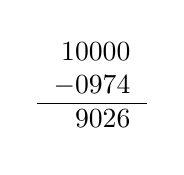
\begin{tikzpicture}
\draw(0,0)node{$
\begin{tabular}{r}
$10000$\\
$-0974$\\
\hline
$9026$
\end{tabular}
$};
\end{tikzpicture}
\end{otherlanguage}
\end{center}
\انتہا{مثال}
\ابتدا{مثال}
دس کے تکملہ کی مدد سے \عددی{974-7852} حاصل کریں۔ 

\ترچھا{جواب}:\quad 
عدد \عددی{7852} کے اساسی تکملہ \عددی{10000-7852=2148} کا \عددی{0974} کے ساتھ مجموعہ لیتے ہوئے: \عددی{0974+2148=3122} آخری حاصل \عددی{1} نہیں پیدا ہوتا، لہٰذا یہ مجموعہ 
 \عددی{4} ہندسوں پر مشتمل ہے؛ اس کے اساسی تکملہ \عددی{10000-3122=6878} کے ساتھ منفی علامت چسپاں کرتے ہوئے \عددی{-6878} کو جواب تسلیم کرتے ہیں۔
\begin{center}
\begin{otherlanguage}{english}
\begin{tikzpicture}
\draw(0,0.5)node[above,yshift=2em]{جواب}node[above,yshift=1em]{$-6878$};
\end{tikzpicture}\quad\quad
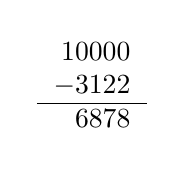
\begin{tikzpicture}
%\draw[thick,black] (-1,-1) grid (1,1);
%\draw [thin, gray,step=0.1](-1,-1) grid (1,1);
\draw(0,0)node{$
\begin{tabular}{r}
$10000$\\
$-3122$\\
\hline
$6878$
\end{tabular}
$};
\end{tikzpicture}\quad\quad
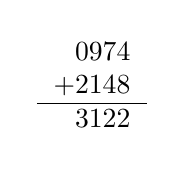
\begin{tikzpicture}
\draw(0,0)node{$
\begin{tabular}{r}
$0974$\\
$+2148$\\
\hline
$3122$
\end{tabular}
$};
\end{tikzpicture}\quad\quad
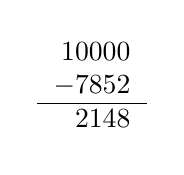
\begin{tikzpicture}
\draw(0,0)node{$
\begin{tabular}{r}
$10000$\\
$-7852$\\
\hline
$2148$
\end{tabular}
$};
\end{tikzpicture}
\end{otherlanguage}
\end{center}
\انتہا{مثال}

ثنائی اعداد بھی بالکل اسی طرح منفی کیے جاتے ہیں۔ان کی بھی دو مثالیں پیش کرتے ہیں۔
	

\ابتدا{مثال}
 اساسی تکملہ کی مدد سے مندرجہ ذیل حاصل کریں۔
 
(ا) \عددی{1011_2-11001_2} اور (ب) \عددی{11001_2-1011_2}

\ترچھا{جواب}:\quad
(ا) چونکہ \عددی{\overline{11001}=00110} ہے، لہٰذا دو کا تکملہ \عددی{00110+1=00111} ہو گا۔ اس کو دوسرے عدد \عددی{01011_2} (جس کی بائیں جانب اضافی \عددی{0} چسپاں کر کے ہندسوں کی تعداد پوری کی گئی) کے ساتھ جمع کرتے ہیں۔
\begin{center}
\begin{otherlanguage}{english}
\begin{tabular}{L}
\phantom{+}01011\\
+00111\\
\midrule
\phantom{+}10010
\end{tabular}
\end{otherlanguage}
\end{center}

بائیں آخری ہندسوں کو جمع کرتے ہوئے حاصل \عددی{1} پیدا نہیں ہوا، لہٰذا اس کا \عددی{2} کا تکملہ لینا ہوگا۔چونکہ \عددی{\overline{10010}=01101} ہے لہٰذا اساسی تکملہ \عددی{01101+1=01110} ہو گا، جس کی بائیں جانب منفی علامت چسپاں کر کے نتیجہ \عددی{-01110_2} حاصل کرتے ہیں۔

\ترچھا{جواب}:\quad (ب) یہاں ایک عدد پانچ ہندسوں پر مشتمل ہے، لہٰذا دوسرے عدد میں بھی پانچ ہندسے پورے کیے جائیں گے۔یوں \عددی{1011} کو \عددی{01011} لکھ کر، اس کے متمم 
 \عددی{\overline{01011}=10100} سے عدد کا اساسی تکملہ \عددی{10100+1=10101} حاصل کر کے، دوسرے عدد کے ساتھ جمع کرتے ہیں۔
 \begin{center}
\begin{otherlanguage}{english}
\begin{tabular}{L}
\phantom{1}1\\
\phantom{+}11001\\
+10101\\
\midrule
\phantom{\,\,}101110
\end{tabular}
\end{otherlanguage}
\end{center}

آخری ہندسے جمع کرتے ہوئے حاصل \عددی{1} پیدا ہوا جس کو نظرانداز کرکے باقی مجموعہ، \عددی{01110_2} ، کو نتیجہ تسلیم کرتے ہیں۔
\انتہا{مثال}


\حصہ{ اساس منفی ایک تکملہ کے ذریعہ اعداد منفی کرنا}\شناخت{حصہ_حساب_منفی_بذریعہ_اساس_منفی_ایک_تکملہ}
اساس منفی ایک تکملہ کی مدد سے بھی \عددی{M-N} حاصل کیا جا سکتا ہے۔ اس کا طریقہ کار درج ذیل ہے جہاں دونوں اعداد میں ہندسوں کی تعداد برابر ہونا لازم ہے ۔
\begin{itemize}
 \item
 دونوں اعداد میں ہندسوں کی تعداد برابر کرنے کی خاطر، کم ہندسوں والے عدد کی بائیں جانب (درکار تعداد کی) اضافی صفریں چسپاں کریں۔ فرض کریں اب ہر عدد میں \عددی{n} ہندسے پائے جاتے ہیں۔ 
 \item
 \عددی{M} کے ساتھ \عددی{N} کا اساس منفی ایک کا تکملہ جمع کر کے \موٹا{مجموعہ} \عددی{M+r^n-1-N} حاصل کریں۔
 \item
 \عددی{M} کی قیمت \عددی{N} کی قیمت سے زیادہ ہونے کی صورت میں، آخری (بائیں) ہندسے جمع کرنے سے حاصل \عددی{1} پیدا ہو گا، جس کی بنا یہ \ترچھا{مجموعہ} \عددی{n+1} ہندسوں پر مشتمل ہو گا اور اس کا بایاں ہندسہ \عددی{1} ہو گا۔اس بائیں ہندسے کو (یعنی حاصل \عددی{1} کو ) نظر انداز کرنے کی بجائے، مجموعہ سے خارج کر کے، \عددی{1} وزن مختص کریں اور \عددی{n} ہندسوں کے باقی مجموعہ کے ساتھ جمع کر کے جواب حاصل کریں۔ اس عمل کو واپسیں آخری حاصل ایک \عددی{(1)} کہتے ہیں۔
 \item
\عددی{M}کی قیمت \عددی{N} کی قیمت سے کم ہونے کی صورت میں، آخری (بائیں) ہندسے جمع کرنے سے حاصل \عددی{1} پیدا \موٹا{نہیں} ہو گا؛ \ترچھا{مجموعہ} منفی عدد کو ظاہر کرے گا، اور \عددی{n} ہندسوں پر مبنی ہو گا۔مجموعے کا اساس منفی ایک کا تکملہ لے کر اس کی بائیں جانب منفی علامت منسلک کر کے جواب حاصل ہو گا۔
\end{itemize}
ان دونوں صورتوں کی وضاحت مثالوں سے ہو گی۔ 

\ابتدا{مثال} 
نو کا تکملہ استعمال کرتے ہوئے \عددی{974-7852} حاصل کریں۔ 

\ترچھا{جواب}:\quad
 عدد \عددی{974} کے بائیں \عددی{0} چسپاں کر کے اس میں ہندسوں کی تعداد پوری کریں اور \عددی{7852} کے اساس منفی ایک کے تکملہ \عددی{9999-7852=2147}کے ساتھ جمع کریں۔
  \begin{center}
\begin{otherlanguage}{english}
\begin{tabular}{L}
\phantom{+}2147\\
+0974\\
\midrule
\phantom{+}3121
\end{tabular}
\end{otherlanguage}
\end{center}
آخری (بائیں) ہندسے جمع کرنے سے حاصل \عددی{1} پیدا نہیں ہوا، لہٰذا مجموعہ چار ہندسوں پر مشتمل ہے۔ اس کے اساس منفی ایک کے تکملہ \عددی{9999-3121=6878} کے بائیں منفی علامت منسلک کر کے جواب \عددی{-6878} حاصل کرتے ہیں۔
\انتہا{مثال}
\ابتدا{مثال}
نو کا تکملہ استعمال کرتے ہوئے \عددی{7852-974} حاصل کریں۔ 

\ترچھا{جواب}\quad
چھوٹے عدد \عددی{974} میں ہندسوں کی تعداد پوری کر کے اس کے اساس منفی ایک کے تکملہ \عددی{9999-0974=9025} کو \عددی{7852} کے ساتھ جمع کرتے ہیں۔
 \begin{center}
\begin{otherlanguage}{english}
\begin{tabular}{L}
\phantom{1}1\\
\phantom{+}7852\\
+9025\\
\midrule
\phantom{\,}16877
\end{tabular}
\end{otherlanguage}
\end{center}
 آخری (بائیں) ہندسے جمع کرتے ہوئے حاصل \عددی{1} پیدا ہوا جس کی بنا یہ مجموعہ \عددی{5} ہندسوں پر مشتمل ہے۔ ہم اس حاصل \عددی{1} کو وزن \عددی{1} مختص کر کے باقی \عددی{4} ہندسوں پر مبنی مجموعہ \عددی{6877} کے ساتھ جمع کر کے جواب \عددی{6877+1=6878} حاصل کرتے ہیں۔
\انتہا{مثال}
اب ہم ثنائی اعداد کی مثال لیتے ہیں۔
\ابتدا{مثال}
 مندرجہ ذیل کو \عددی{1} کے تکملہ کی مدد سے حل کریں۔

(ا) \عددی{101110_2-11011_2}، (ب) \عددی{11011_2-101110_2} 

\ترچھا{حل}:\quad
 (ا) منفی ہونے والے عدد میں ہندسوں کی تعداد پوری کر کے اس کا متمم:
 \begin{align*}
 \overline{011011}=100100
 \end{align*}

دوسرے عدد کے ساتھ جمع کرتے ہیں۔
 \begin{center}
\begin{otherlanguage}{english}
\begin{tabular}{L}
\phantom{1}1\\
\phantom{+}101110\\
+100100\\
\midrule
\phantom{\,\,}1010010
\end{tabular}
\end{otherlanguage}
\end{center}
آخری حاصل \عددی{1} کو باقی عدد سے علیحدہ کر کے اسے \عددی{1} کا وزن مختص کر کے (یعنی اس کو اکائی تصور کر کے)، دائیں چھ ہندسوں پر مشتمل مجموعہ \عددی{010010} کے ساتھ جمع کرتے ہوئے جواب حاصل کرتے ہیں۔
 \begin{center}
\begin{otherlanguage}{english}
\begin{tabular}{R}
010010\\
+1\\
\midrule
010011
\end{tabular}
\end{otherlanguage}
\end{center}
متمم \عددی{\overline{101110}=010001} کو دوسرے عدد کے ساتھ جمع کرتے ہیں۔
 \begin{center}
\begin{otherlanguage}{english}
\begin{tabular}{R}
010001\\
+011011\\
\midrule
101100
\end{tabular}
\end{otherlanguage}
\end{center}
چونکہ آخری حاصل صفر ہے، لہٰذا مجموعے کے متمم \عددی{\overline{101100}=010011} کے ساتھ منفی کی علامت چسپاں کر کے جواب \عددی{-010011_2} حاصل کرتے ہیں۔
 \انتہا{مثال}
 
 
\حصہ{مثبت اور منفی اعداد}
روز مرہ زندگی میں مثبت اعداد لکھتے ہوئے انہیں بغیر کسی علامت کے، یا مثبت علامت \عددی{(+)} کے ساتھ لکھا جاتا ہے، البتہ منفی اعداد کے ساتھ منفی علامت \عددی{(-)} ضرور لکھی جاتی ہے۔یوں درج ذیل اعداد درست لکھے گئے ہیں۔
\begin{align*}
+3025, \quad \quad 3025, \quad \quad -3025
\end{align*}
کسی بھی عدد کے مثبت یا منفی ہونے کو اس عدد کی علامت کہتے ہیں۔ یوں، وہ اعداد جو مثبت علامت \عددی{(+)} یا منفی علامت \عددی{(-)} رکھتے ہوں علامت دار اعداد کہلاتے ہیں، اور جن کی علامت نہ ہو بے علامت اعداد کہلاتے ہیں۔ اعداد کو ان کی علامت اور قدر سے ظاہر کرنے کو علامت دار قدر اظہار کہتے ہیں۔ 

کمپیوٹر ثنائی اعداد ، \عددی{0} اور \عددی{1}، استعمال کرتا ہے، اور ہر معلومات کو انہیں سے ظاہر کرتا ہے۔روایتاً مثبت علامت \عددی{(+)} کو \عددی{0} (صفر ) اور نفی علامت \عددی{(-)} کو \عددی{1} (ایک) سے ظاہر کیا جاتا ہے۔علامت عدد کی بائیں جانب لکھی جاتی ہے۔ یوں \عددی{+5_{10}} کو چار ثنائی ہندسوں سے ظاہر کرتے ہوئے، بایاں ہندسہ مثبت علامت \عددی{(+)} کو جبکہ باقی تین ہندسے \عددی{5} کو ظاہر کریں گے۔ اسی طرح \عددی{-5_{10}} کو آٹھ ثنائی ہندسوں سے ظاہر کرتے ہوئے، بایاں ہندسہ منفی علامت \عددی{(-)} کو جبکہ باقی سات ہندسے \عددی{5} کو ظاہر کریں گے۔ 
\begin{align*}
\underbrace{0}_{+}\underbrace{1\,\,\,0\,\,\,1}_{\,\,5_{10}}\quad \quad \quad \underbrace{1}_{-}\underbrace{0\,\,\,0\,\,\,0\,\,\,0\,\,\,1\,\,\,0\,\,\,1}_{5_{10}}
\end{align*}


ایک دلچسپ حقیقت پر غور کریں۔اگر ہم \عددی{1101_2} میں بایاں ہندسہ علامت تصور کریں تب یہ \عددی{-5_{10}} کو ظاہر کرے گا، لیکن اگر ہم چاروں ہندسوں کو ایک عدد تصور کریں تب یہ \عددی{D_{16}} یا \عددی{13_{10}} کو ظاہر کرتا ہے۔

یہ جاننا ضروری ہے، آیا ثنائی اعداد کا بایاں ہندسہ علامت کو ظاہر کرتا ہے یا یہ عدد کا حصہ ہے؛ یہ فیصلہ اعداد استعمال کرنے والے پر ہے۔کمپیوٹر استعمال کرتے وقت آپ فیصلہ کرتے ہیں کہ علامت دار یا بے علامت (غیر علامت دار)
 اعداد استعمال کریں گے۔ جدول \حوالہ{جدول_حساب_علامت_دار_چار} میں چار ثنائی ہندسوں پر مشتمل علامت دار اعداد دکھائے گئے ہیں۔ آپ دیکھ سکتے ہیں کہ صفر کو دو مختلف طریقوں سے ظاہر کیا جا سکتا ہے، ان میں ایک مثبت اور دوسرا منفی ہے!
\begin{table}
\caption{چار ہندسوں کے علامت دار اعداد}
\label{جدول_حساب_علامت_دار_چار}
\centering
\begin{tabular}{CC}
\toprule
\text{ثنائی} & \text{علامت دار}\\
\midrule
0111_2 & +7_{10}\\
0110_2&+6_{10}\\
0101_2&+5_{10}\\
0100_2&+4_{10}\\[0.5em]
0011_2&+3_{10}\\
0010_2&+2_{10}\\
0001_2&+1_{10}\\
0000_2&+0_{10}\\[0.5em]
1000_2&-0_{10}\\
1001_2&-1_{10}\\
1010_2&-2_{10}\\
1011_2&-3_{10}\\[0.5em]
1100_2&-4_{10}\\
1101_2&-5_{10}\\
1110_2&-6_{10}\\
1111_2&-7_{10}\\
\bottomrule
\end{tabular}
\end{table}

اس جدول میں چار ثنائی ہندسوں سے اعداد لکھے گئے؛ کمپیوٹر میں اعداد، عموماً، ایک بائٹ استعمال کرتے ہوئے لکھا جاتا ہے۔ ایک بائٹ \عددی{8} ثنائی ہندسوں کو کہتے ہیں۔ علامت دار اعداد کو بائٹ میں لکھتے ہوئے، دائیں سات ہندسے عدد کی قدر جبکہ بایاں آخری ہندسہ اس کی علامت ظاہر کرے گا۔
\begin{align*}
00000101_2&=+5_{10}\\
01111111_2&=+127_{10}\\
10000101_2&=-5_{10}\\
11111111_2&=-127_{10}\\
00000000_2&=+0_{10}\\
10000000_2&=-0_{10}
\end{align*}
ان اعداد میں بھی مثبت اور منفی صفر پایا گیا؛ روز مرہ زندگی میں صفر کو ہم مثبت تصور کرتے ہیں۔

اتنا کچھ کہنے کے بعد آپ کو بتاتا چلوں کہ، کمپیوٹر میں منفی اعداد کو  علامت دار قدر اظہار میں نہیں بلکہ علامت دار و \عددی{1} کے تکملہ یا علامت دار و \عددی{2} کے تکملہ نظام میں رکھا اور استعمال کیا جاتا ہے۔اگلے حصہ میں ان نظام پر غور ہو گا۔

\حصہ{علامت دار  و   تکملہ نظام}
کمپیوٹر میں عددی برقیات کی مدد سے اعداد جمع یا منفی کیے جاتے ہیں۔ یہ اعمال اساسی تکملہ یا اساس منفی ایک  تکملہ (حصہ \حوالہ{حصہ_حساب_منفی_بذریعہ_اساسی_تکملہ} اور حصہ \حوالہ{حصہ_حساب_منفی_بذریعہ_اساس_منفی_ایک_تکملہ} دیکھیں) استعمال کرتے ہوئے زیادہ خوش اسلوبی سے سرانجام دیے جاتے ہیں۔

 کمپیوٹر چونکہ ثنائی اعداد استعمال کرتا ہے، لہٰذا اس میں منفی اعداد \عددی{1} کے تکملہ یا \عددی{2} کے تکملہ میں لکھے جاتے ہیں۔جدول \حوالہ{جدول_حساب_علامت_دار_تکملہ_ایک_دو} میں چار ثنائی ہندسی (چار بِٹ)  \اصطلاح{علامت دار  }\فرہنگ{علامت دار}\حاشیہب{signed}\فرہنگ{signed} اعداد کا \عددی{1} کا تکملہ اور \عددی{2} کا تکملہ روپ پیش کیا گیا ہے۔
\begin{table}
\caption{علامت دار ایک کا تکملہ اور دو کا تکملہ اعداد}
\label{جدول_حساب_علامت_دار_تکملہ_ایک_دو}
\centering
\begin{tabular}{CCCC}
\toprule
\text{اعشاری عدد} & \text{علامت دار قدر} & \text{علامت دار ایک کا تکملہ} & \text{علامت دار دو کا تکملہ}\\
\midrule
+7&0111&0111&0111\\
+6&0110&0110&0110\\
+5&0101&0101&0101\\
+4&0100&0100&0100\\[0.5em]
+3&0011&0011&0011\\
+2&0010&0010&0010\\
+1&0001&0001&0001\\
+0&0000&0000&0000\\[0.5em]
-0&1000&1111&\text{نہیں پایا جاتا}\\
-1&1001&1110&1111\\
-2&1010&1101&1110\\
-3&1011&1100&1101\\[0.5em]
-4&1100&1011&1100\\
-5&1101&1010&1011\\
-6&1110&1001&1010\\
-7&1111&1000&1001\\
-8&\text{نہیں پایا جاتا}&\text{نہیں پایا جاتا}&1000\\
\bottomrule
\end{tabular}
\end{table}

جدول \حوالہ{جدول_حساب_علامت_دار_تکملہ_ایک_دو} سے آپ دیکھ سکتے ہیں کہ مثبت عدد، ثنائی ہندسوں میں ایک ہی طریقہ سے لکھا جاتا ہے، جبکہ منفی عدد تین طریقوں سے لکھا جا سکتا ہے۔یوں تینوں طریقوں میں مثبت عدد کو سادہ ثنائی عدد لکھیں۔

	مثبت عدد \عددی{+x} کی علامت دار روپ میں \اصطلاح{ علامتی بِٹ }\فرہنگ{علامتی بِٹ}\حاشیہب{sign bit}\فرہنگ{sign bit} \عددی{0} سے \عددی{1} کرنے سے \عددی{-x} کا \قول{علامت دار روپ}  حاصل ہو گا۔یوں \عددی{-5} کو علامت دار روپ میں لکھنے کی خاطر \عددی{+5} کو علامت دار روپ \عددی{0101_2} میں لکھ کر علامتی بِٹ \عددی{1} کرنے سے \عددی{-5} کی علامت دار روپ \عددی{1101_2} حاصل ہو گی۔
	
منفی عدد \عددی{-x} کو\اصطلاح{ علامت دار ایک کے تکملہ روپ } میں لکھنے کی خاطر \عددی{+x} کو علامت دار ثنائی عدد (یعنی سادہ ثنائی روپ میں) لکھ کر اس کا \عددی{1} کا تکملہ لیں۔یاد رہے کہ \عددی{1} کا تکملہ حاصل کرتے ہوئے ثنائی عدد کے ہر ہندسہ (بمع علامتی بِٹ) کا متمم لینا ہو گا۔ یوں \عددی{-5} کو علامت دار ایک کے تکملہ روپ میں لکھنے کی خاطر \عددی{+5} کو \عددی{0101_2} لکھ کر متمم لیں جو درکار روپ \عددی{1010_2} دے گا۔

منفی عدد \عددی{-x} کو علامت دار دو کے تکملہ روپ میں لکھنے کی خاطر \عددی{+x} کو علامت دار ثنائی عدد (یعنی سادہ ثنائی روپ میں) لکھ کر اس کا \عددی{2} کا تکملہ لیں۔یاد رہے کہ \عددی{2} کا تکملہ حاصل کرتے ہوئے ثنائی عدد کے ہر ہندسہ (بمع علامتی بِٹ) کا متمم لینا ہو گا۔ یوں \عددی{-5} کو علامت دار دو کے تکملہ روپ میں لکھنے کی خاطر \عددی{+5} کو \عددی{0101_2} لکھ کر دو کا تکملہ لیں جو درکار روپ \عددی{1011_2} دے گا۔

\حصہء{سوالات}
%Q2.1
\ابتدا{سوال}
درج ذیل ثنائی مجموعے حاصل کریں۔ان سوالات کو عشری  روپ میں بھی حل کریں۔جوابات کا موازنہ کریں۔
\begin{multicols}{4}
\begin{enumerate}[a.]

\item  
 \(110+101\)  
\item 
 \(11+101\) 

\item  
 \(1011+1101\)  
\item 
 \(1101+1001\)   

\item  
 \(101+1011\)  
\item 
 \(101+1111\)  
\end{enumerate}
\end{multicols}
جواب:ثنائی \عددی{1011}، \عددی{1000}، \عددی{11000}، \عددی{10110}، \عددی{10000}، \عددی{10100}؛ 
اعشاری   \عددی{11}، \عددی{8}، \عددی{24}، \عددی{22}، \عددی{16}، \عددی{20}
\انتہا{سوال}
\ابتدا{سوال}
%Q2.2
درج ذیل ثنائی اعداد کے سوالات حل کریں۔ان سوالات کو اعشاری روپ میں بھی حل کریں۔جوابات کا موازنہ کریں۔
\begin{multicols}{4}
\begin{enumerate}[a.]

\item  
 \(110-101\)  
\item 
 \(111-101\) 

\item  
 \(1111-1101\)  
\item 
 \(1101-1001\)   

\item  
 \(101-1011\)  
\item 
 \(101-1111\)
\end{enumerate}
\end{multicols}
جواب: ثنائی  \عددی{1}، \عددی{10}، \عددی{10}،  \عددی{100}، \عددی{-110}، \عددی{-1010}؛
 اعشاری  \عددی{1}، \عددی{2}، \عددی{2}، \عددی{4}،  \عددی{-6}، \عددی{-10}
\انتہا{سوال}
\ابتدا{سوال}
%Q2.3
درج ذیل ثنائی اعداد کے سوالات حل کریں۔انہیں سوالات کو اعشاری روپ میں بھی حل کریں۔جوابات کا موازنہ کریں۔
\begin{multicols}{4}
\begin{enumerate}[a.]
\item  
 \(110-10.1\)  
\item 
 \(101-10.1\) 

\item  
 \(11.11-1.101\)  
\item 
 \(110.1-10.01\)   

\item  
 \(101.011-10.11\) 
\item 
 \(111.1-11.01\)
\end{enumerate}
\end{multicols}
جواب: ثنائی  \عددی{11.1}، \عددی{10.1}، \عددی{10.001}، \عددی{100.01}، \عددی{10.101}، \عددی{100.01}
\انتہا{سوال}
\ابتدا{سوال}
%Q2.4
درج ذیل اعشاری سوالات کو ثنائی روپ میں تبدیل کر کے حل کریں۔
\begin{multicols}{4}
\begin{enumerate}[a.]

\item  
 \(64+32\)  
\item  
 \(256-128\) 
\item  
 \(121.2-94.3\) 
\item  
 \(36.09+22.24\)  
\item  
 \(1024-63\) 
\item  
 \(2056+1024\)    
\end{enumerate}
\end{multicols}
جواب:  \عددی{1100000}، \عددی{10000000}، \عددی{11010.1110}، \عددی{111010.010}، \عددی{1111000001}، \عددی{110000001000}
\انتہا{سوال}
\ابتدا{سوال}
%Q2.5
درج ذیل اعشاری اعداد کا تکملہ نو اور تکملہ دس حاصل کریں۔
\begin{multicols}{4}
\begin{enumerate}[a.]
\item  
 \(6\)  
\item   
 \(8\) 
\item  
 \(19\)  
\item   
 \(205\) 
\item  
 \(3160029\) 
\item   
 \(9807568\) 
\item  
 \(0.63\)  
\item   
 \(39.09\) 
\item  
 \(3093.9801\) 
\item   
 \(23409.65487\) 
\end{enumerate}
\end{multicols}
جواب:  تکملات نو  \عددی{3}، \عددی{1}، \عددی{80}، \عددی{794}، \عددی{6839970}، \عددی{0192431}؛ تکملات دس  \عددی{4}، \عددی{2}، \عددی{81}، \عددی{795}، \عددی{6839971}، \عددی{0192432}
\انتہا{سوال}
\ابتدا{سوال}
%Q2.6
درج ذیل ثنائی اعداد کا (اتنے  ہی ہندسوں میں)  تکملہ ایک اور تکملہ دو حاصل کریں۔
\begin{multicols}{4}
\begin{enumerate}[a.]

\item  
 \(1011\)  
\item   
 \(1001\) 
\item  
 \(111101\) 
\item   
 \(10101010\) 
\item  
 \(11.11\)  
\item   
 \(1101.0011\) 
\end{enumerate}
\end{multicols}
جواب: تکملات ایک  \عددی{0100}، \عددی{0110}، \عددی{000010}، \عددی{01010101}؛  تکملات دو  \عددی{0101}، \عددی{0111}، \عددی{000011}، \عددی{01010110}
\انتہا{سوال}
\ابتدا{سوال}
%Q2.7
درج ذیل اعشاری سوالات کو تکملہ نو اور تکملہ دس استعمال کرتے ہوئے حل کریں۔ سادہ طریقے سے حاصل جوابات کے ساتھ موازنہ کریں۔
\begin{multicols}{3}
\begin{enumerate}[a.]

\item  
 \(9-4\)  
\item   
 \(16-9\) 
\item  
 \(23.9-13\) 
\item  
 \(555.078-303.93\) 
\item  
 \(0.555-0.045\) 
\item  
 \(1000-909.5301\) 
\end{enumerate}
\end{multicols}
\انتہا{سوال}
\ابتدا{سوال}
%Q2.8
درج ذیل ثنائی سوالات کو تکملہ ایک اور تکملہ دو سے حل کریں۔ سادہ ثنائی طریقے سے حاصل جوابات کے ساتھ موازنہ کریں۔
\begin{multicols}{3}
\begin{enumerate}[a.]
\item  
 \(11-10\)  
\item  
 \(1101-1010\) 
\item  
 \(11.10-10.11\) 
\item  
 \(1101.01-1001.1\) 
\item  
 \(101-1010\) 
\item  
 \(0.11-1101.11\) 
\end{enumerate}
\end{multicols}
\انتہا{سوال}
\ابتدا{سوال}
%Q2.9
درج ذیل اعشاری سوالات کو ثنائی روپ میں تبدیل کر کے حل کریں- جواب کو واپس اعشاری روپ میں تبدیل کر کے اعشاری طریقے سے حاصل جواب کے ساتھ موازنہ کریں۔
\begin{multicols}{4}
\begin{enumerate}[a.]
\item 
 \(3\times 9\)   
\item 
 \(31\times 23\)   
\item 
 \(15\times 3.625\)  
\item  
 \(1024\times 16\) 
\item 
 \(2048\times 2048\) 
\item 
 \(65.75\times 11.625\) 
\end{enumerate}
\end{multicols}
\انتہا{سوال}
%================

